\documentclass[subsection=false]{beamer}
\setbeamertemplate{footline}[frame number] % numerar slides
\setbeamertemplate{navigation symbols}{} % retirar barra de navega��o

\mode<presentation>
\usetheme{Singapore}

\ifdefined\hyperref  

\usepackage[brazil]{babel}
\usepackage[latin1]{inputenc}
\usepackage{graphicx}
\usepackage{subcaption}  
\usepackage{pgfpages}
\usepackage{ifpdf}   
\usepackage{multimedia}  
\usepackage{color}   
\usepackage{url} 
\usepackage{hyperref}
\usepackage{lastpage}
\usepackage{listings}

\lstset{%
	linewidth=\textwidth,%framed box is the text size 
	xleftmargin=.25in,
	xrightmargin=.25in, 
	frame=trbl, 
	columns=flexible, 
	captionpos=t, 
	upquote=false,
	basicstyle=\footnotesize\ttfamily,
	firstnumber=1,% 
	numberfirstline=false,% 
	numbers=left,%
	numberstyle=\tiny,% 
	stepnumber=5,%
	numbersep=5pt,% 
	backgroundcolor=\color{green!15},% 
	tabsize=4,% 
	keywordstyle=\color{green!65!black},% 
	commentstyle=\color{blue},% 
	stringstyle=\color{magenta},% 
	breaklines=true,% 
	emph={label},%
	abovecaptionskip=10pt,% 
	belowcaptionskip={\abovecaptionskip},%
	showstringspaces=false, 
	literate={�}{{\^{E}}}1
}%

\pgfdeclareimage[width=0.85cm, height=1.10cm]{ufpa}{Figures/logo_ufpa}
\logo{\pgfuseimage{ufpa}}

\hypersetup{
	pdftitle={ASR e TTS Embarcado para Controle de TV}
	pdfauthor={Cassio Trindade Batista}
}
\fi

\title[ASR + TTS: Controle de Equipamentos Eletr�nicos\hspace{2.10cm}\thepage/\pageref{LastPage}]
{\Large Uso de Reconhecedor e Sintetizador de Voz Embarcados para
Controle de Equipamentos Eletr�nicos via Luz Infravermelha}
%{Uso de Reconhecedor e Sintetizador de Voz para Controle de Equipamentos Eletr�nicos}

\author[Cassio, Pedro, Gabriel e Thiago]{
\small
Cassio Trindade Batista\\
Gabriel Peixoto de Carvalho\\
Pedro Henrique C. F. Soares\\
Thiago Barros Coelho}

\institute{
\scriptsize
Universidade Federal do Par�\\
Instituto de Tecnologia\\
Faculdade de Engenharia da Computa��o e Telecomunica��es\\
Disciplina: Projetos de Hardware e Interfaceamento\\
Professores: Jeferson Leite e Adalbery Castro\\
\begin{figure}
	
\includegraphics[width=.11\textwidth]{Figures/logo_ufpa}
\end{figure}
\vspace{-.6cm}
}
\date{\small{25 de junho de 2015}}

\begin{document}
\begin{frame}[plain]
	\titlepage
\end{frame}

\section{Introdu��o}
\subsection{Introdu��o}
\begin{frame}{Introdu��o}
\begin{itemize}
	\item 23\% dos brasileiros possuem necessidades especiais
	\item Teclado e Mouse: Exclus�o digital
	\item Dificuldade em controles convencionais para deficientes
	\item Acessibilidade: Novas formas de controle
\end{itemize}
\begin{figure}
	
\includegraphics[width=.7\textwidth]{Figures/accessibility}
\end{figure}
\end{frame}

\section{Objetivos}
\subsection{Objetivos}
\begin{frame}{Objetivos}
\textcolor{blue}{Objetivo Geral}: Controle de TV via \textit{smartphone} 
atrav�s da voz \medskip
\begin{itemize}
	\item BeagleBone Black\smallskip
	\begin{itemize}
		\item Servidor de reconhecimento de fala \smallskip
		\item Servidor de s�ntese de fala \smallskip
		\item Servidor LAMP de armazenamento de comandos \medskip
	\end{itemize}
	\item Arduino UNO\smallskip
	\begin{itemize}
		\item Transmissor de Sinais Infravermelhos (IR LED) \smallskip
		\item Receptor de Sinais Infravermelhos (IR Receiver) \medskip
	\end{itemize}
	\item Android\smallskip
	\begin{itemize}
		\item Microfone (cliente)
	\end{itemize}
\end{itemize}
\end{frame}

\begin{frame}{Esquem�tico do Projeto}
\begin{figure}
	\includegraphics[width=\textwidth]{Figures/schematic}
\end{figure}
\end{frame}

\begin{frame}{Cliente Android}
\begin{figure}
	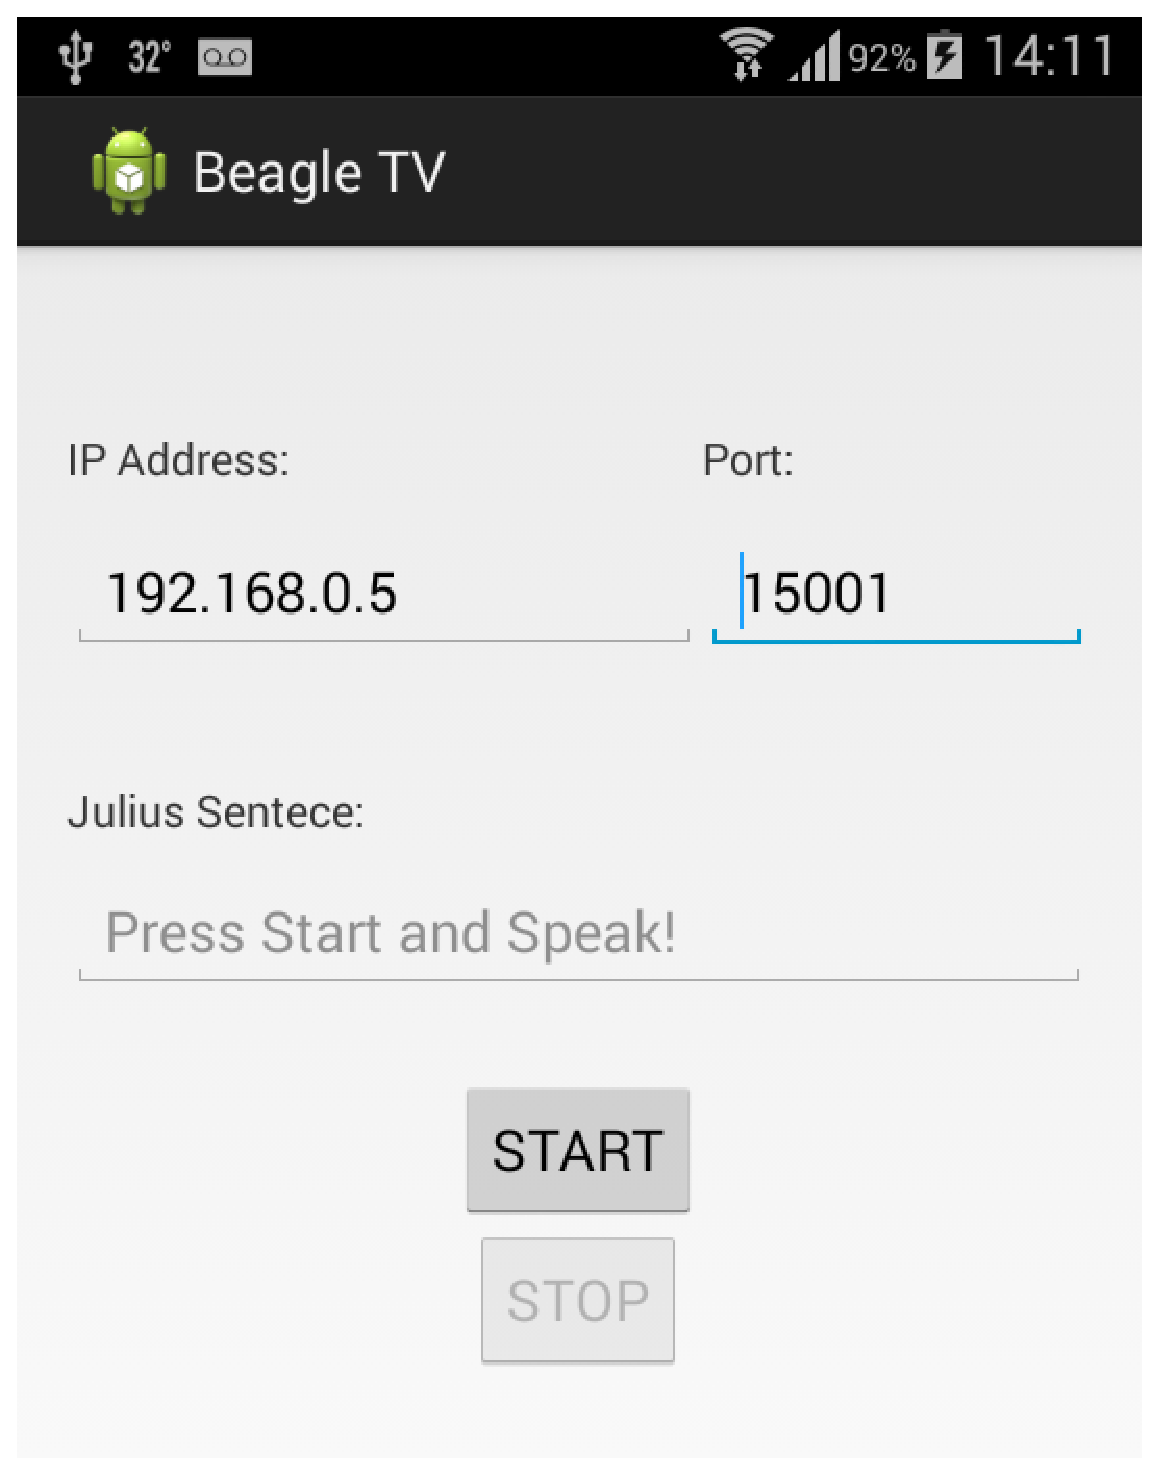
\includegraphics[width=.5\textwidth]{Figures/app}
\end{figure}
\end{frame}

\section{Teoria}
\subsection{Teoria}
\begin{frame}{Reconhecimento \textit{vs.} S�ntese}
\begin{figure}
	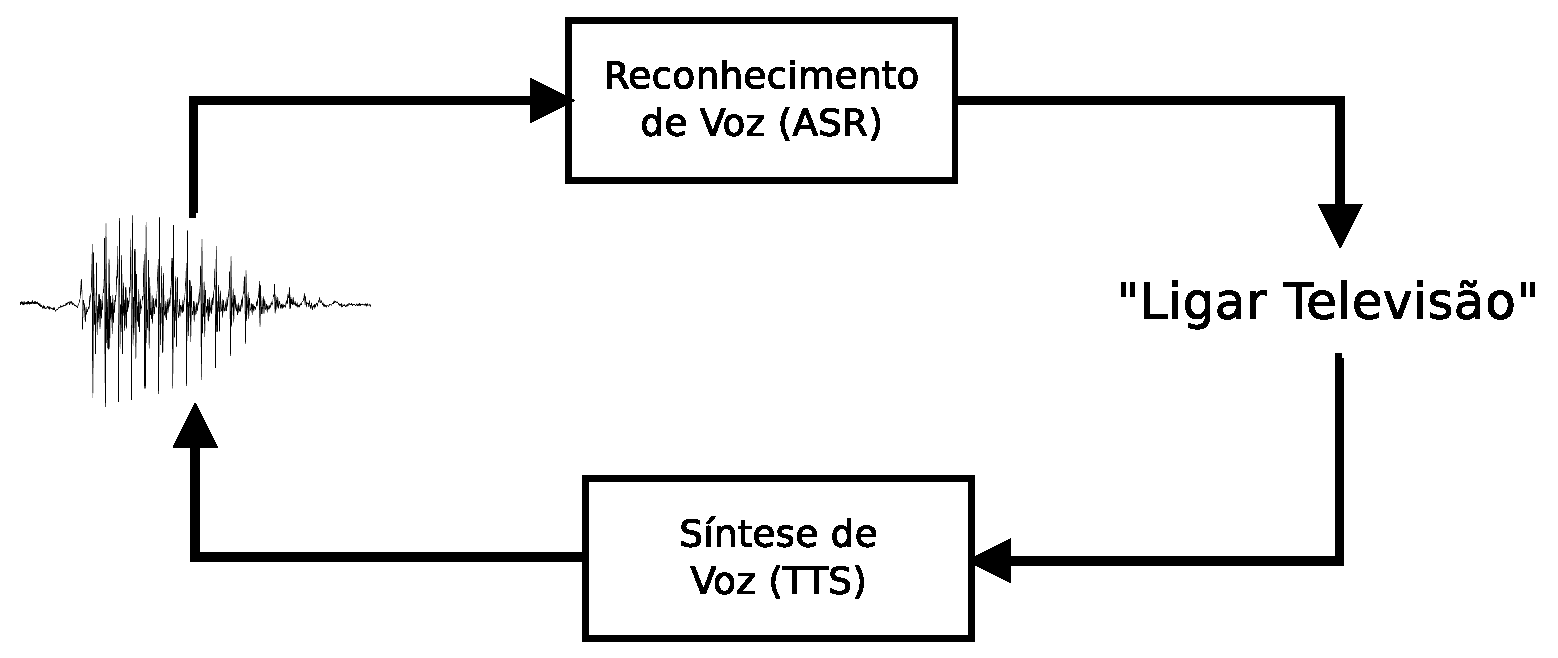
\includegraphics[width=\textwidth]{Figures/asr_tts}
\end{figure}
\end{frame}

\begin{frame}{Reconhecimento \textit{vs.} S�ntese}
\begin{figure}
	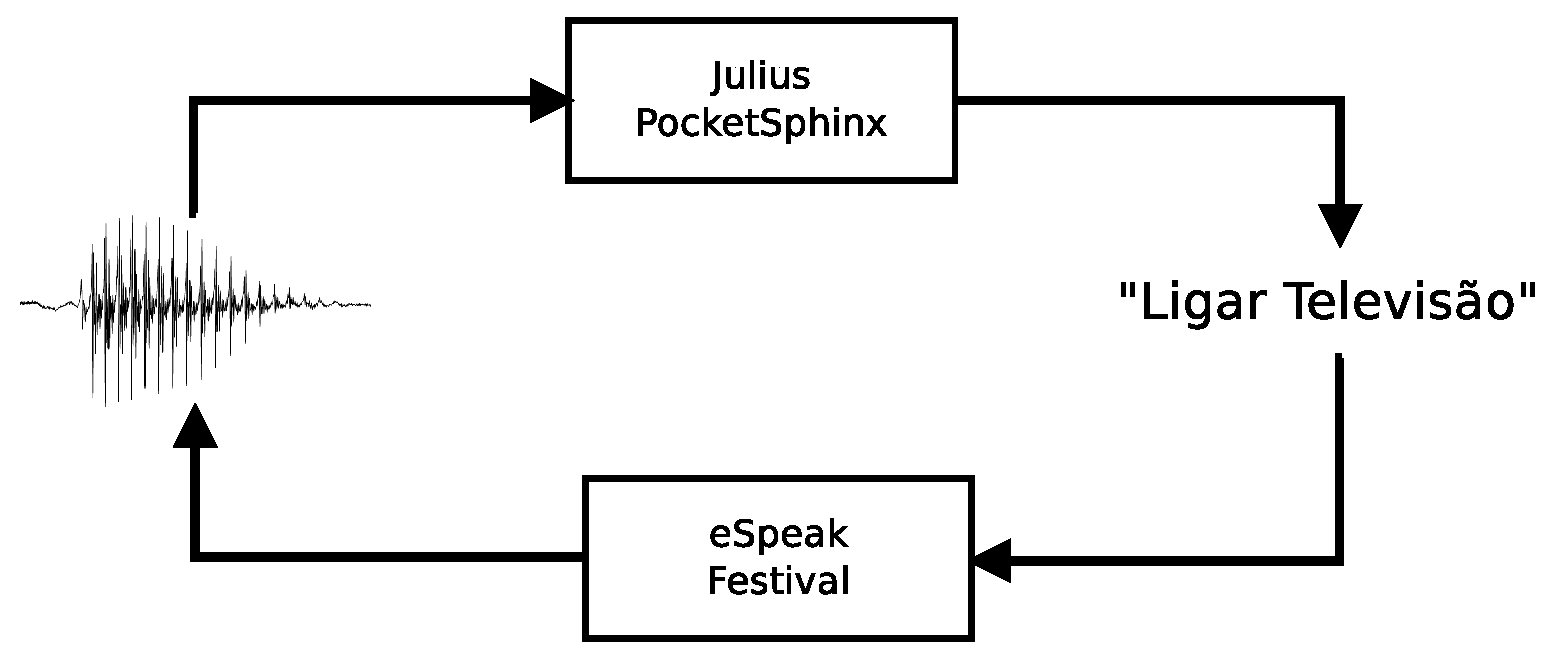
\includegraphics[width=\textwidth]{Figures/asr_tts_soft}
\end{figure}
\end{frame}

\begin{frame}{ASR: Esquem�tico}
ASR: \textit{Automatic Speech Recognition}
\begin{figure}
	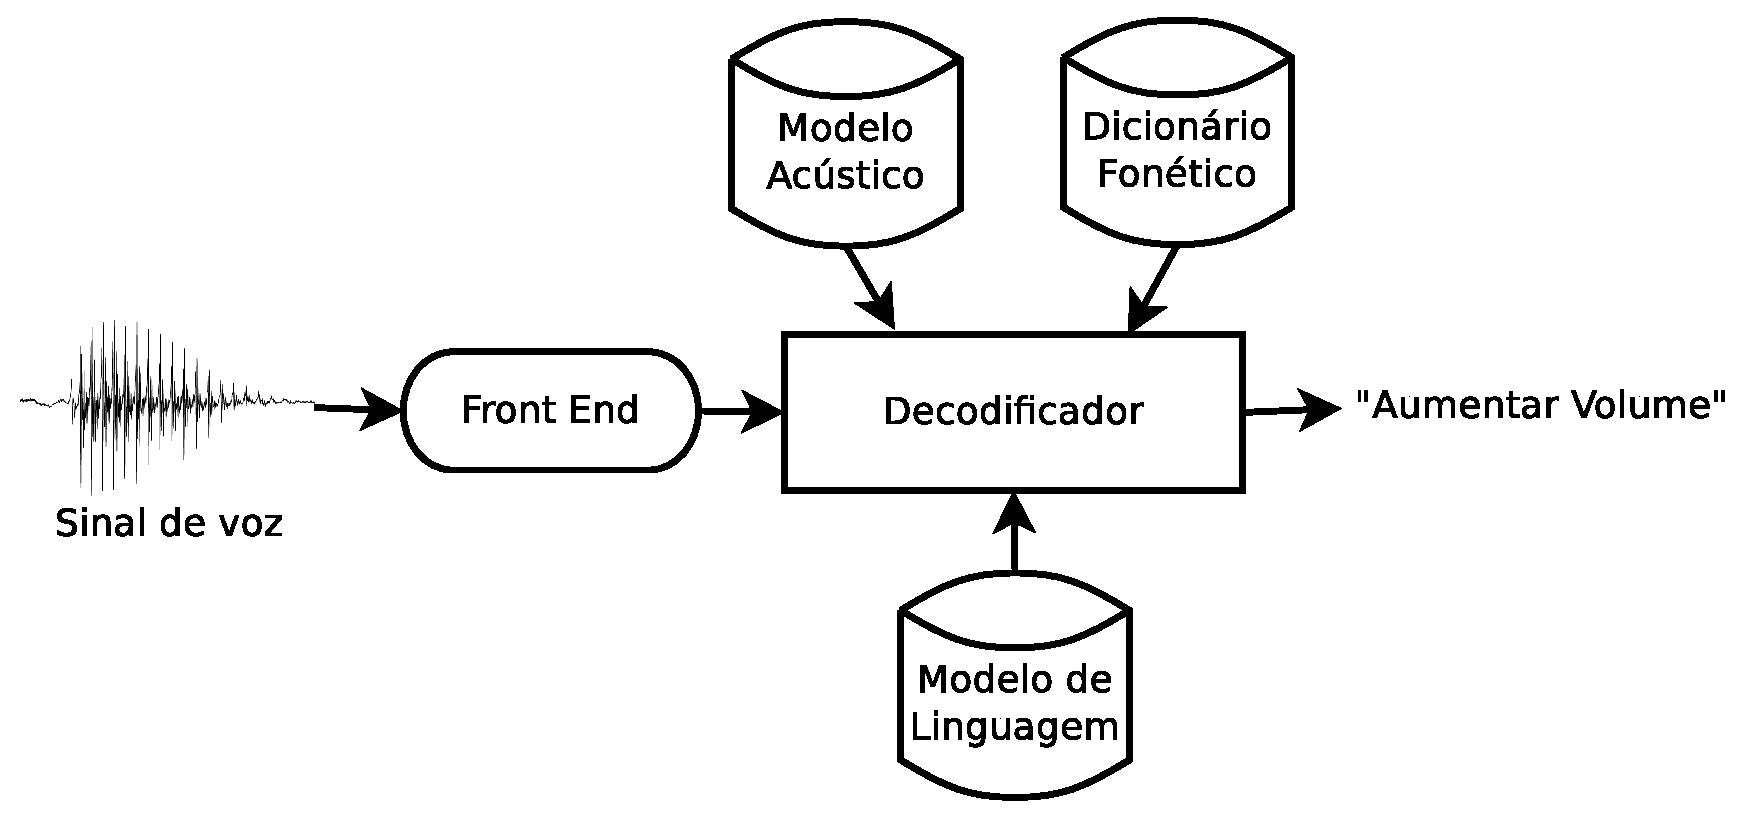
\includegraphics[width=\textwidth]{Figures/asr_sch}
\end{figure}
\end{frame}

\begin{frame}[fragile]{ASR: Gram�tica e Dicion�rio}
\begin{lstlisting}[label={lst:gram}]
<s> aumentar volume </s>
<s> diminuir volume </s>
<s> canal mais </s>
<s> canal menos </s>
<s> ligar televis�o </s>
<s> desligar televis�o </s>
\end{lstlisting}
\begin{lstlisting}[label={lst:dict}]
aumentar	a u~ m e~  t a X  
diminuir	dZ i~ m i~ n u j X  
volume		v o l u~ m i  
canal		k a n a w  
mais		m a j s
menos		m e~ n u s
televis�o	t e l e v i z a~ w~   
\end{lstlisting}
\end{frame}

\begin{frame}{PWM: Modula��o por Largura de Pulso}
\begin{figure}
	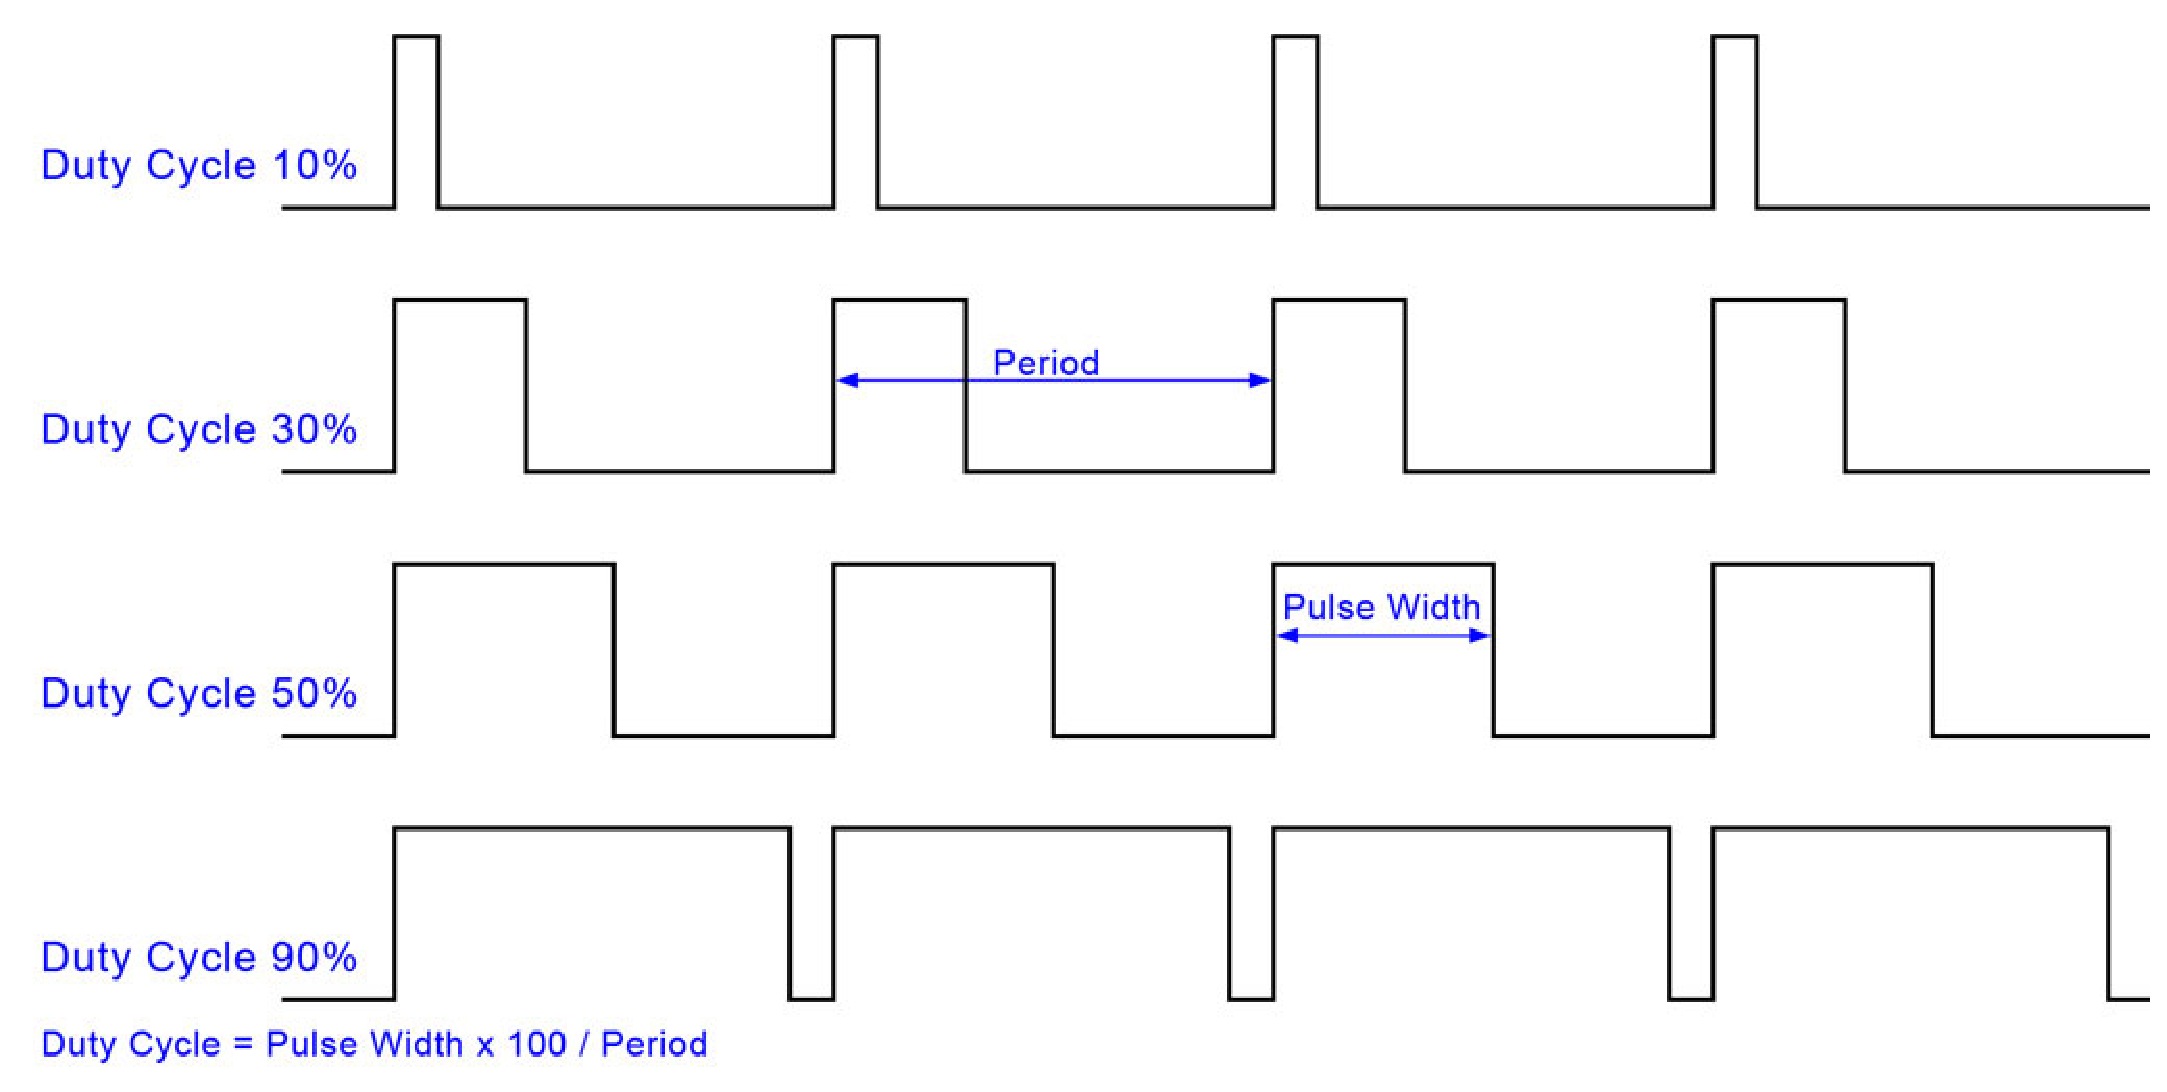
\includegraphics[width=.95\textwidth]{Figures/pwm}
\end{figure}
\end{frame}

\begin{frame}{PWM: Tens�o M�dia}
\begin{figure}
	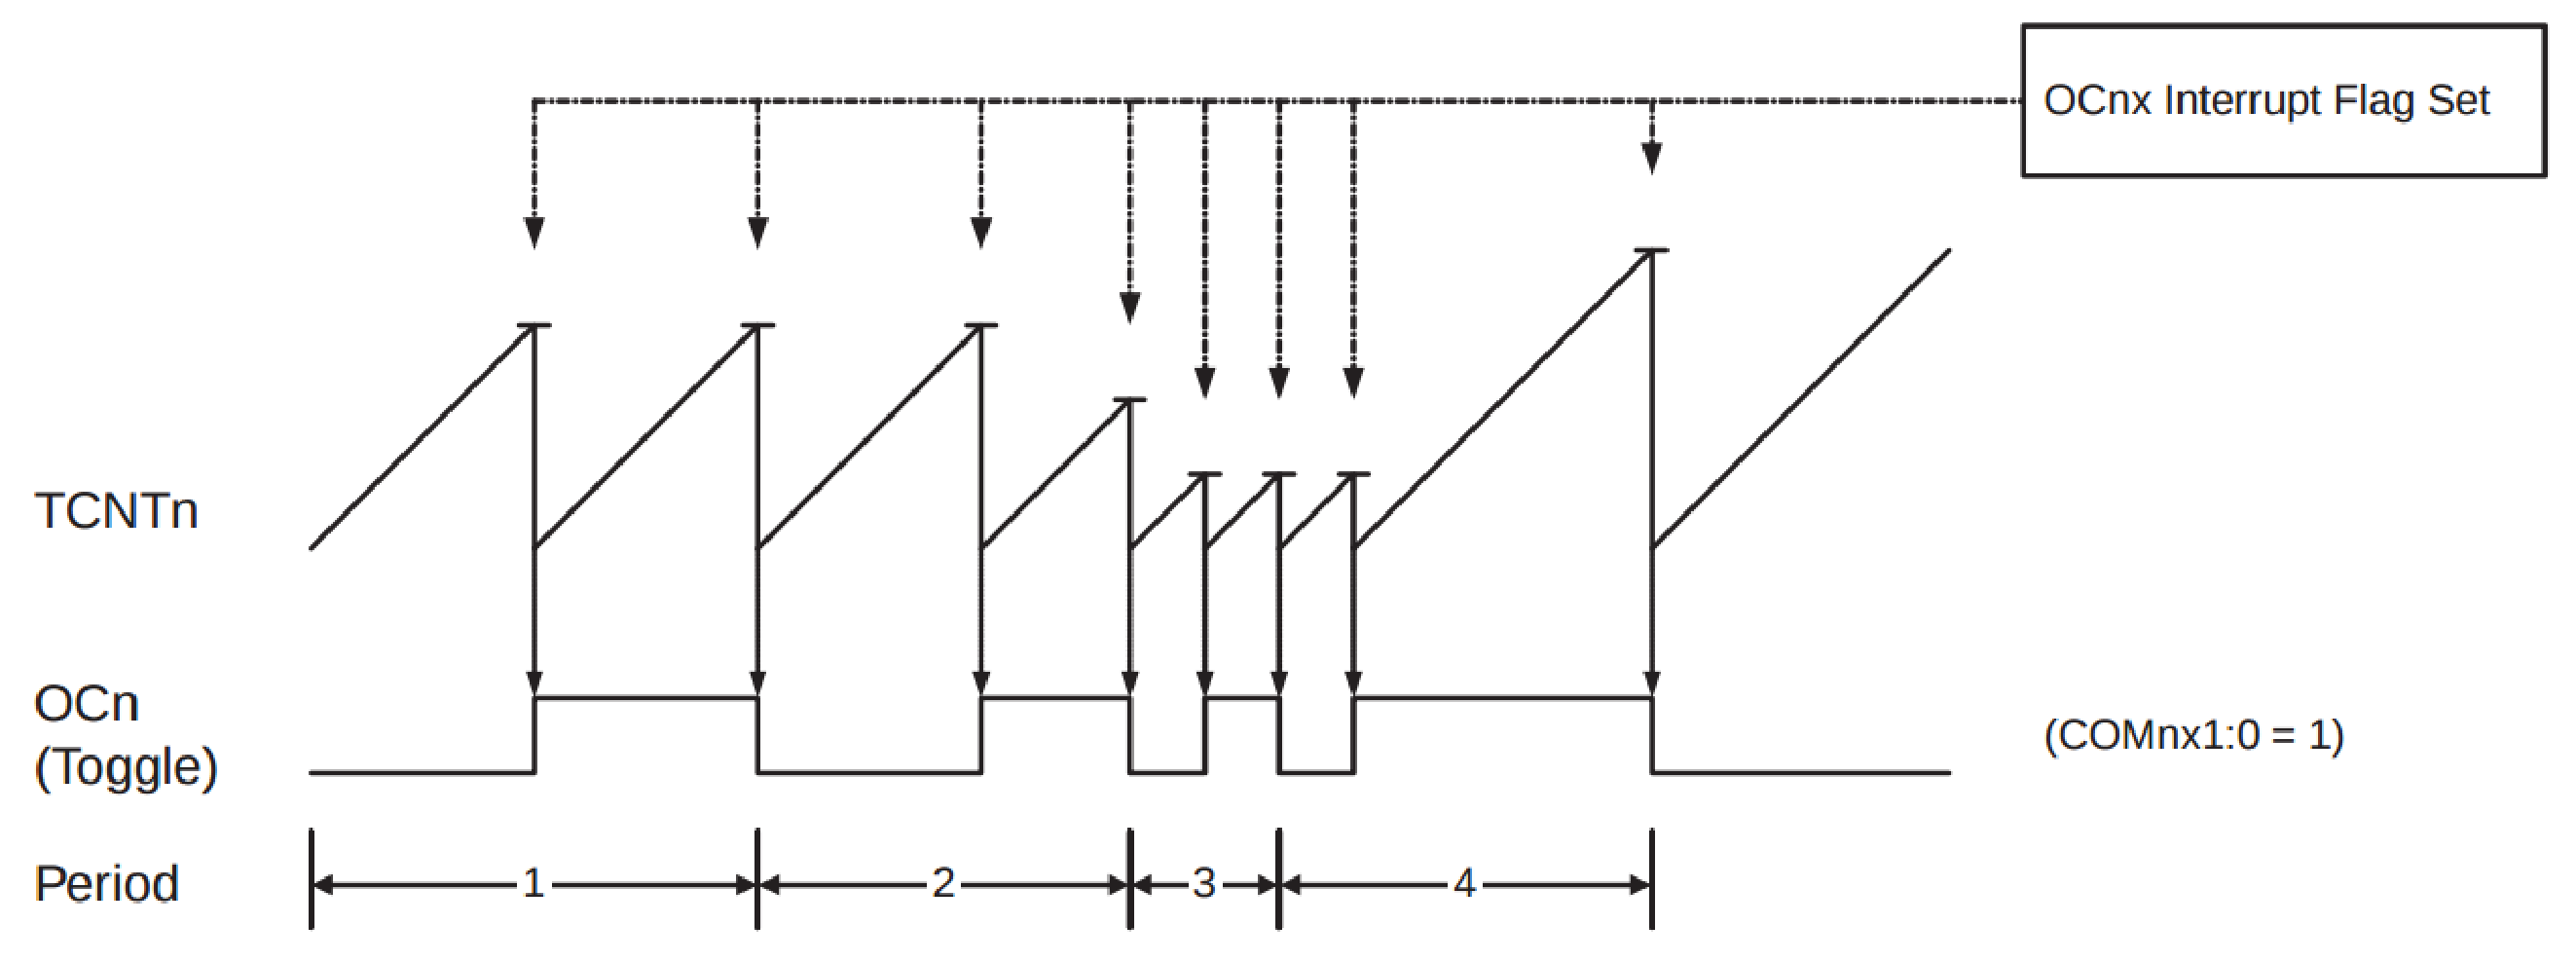
\includegraphics[width=\textwidth]{Figures/pwm_avgvolt}
	%\caption{Datasheet do arduino}
\end{figure}
\end{frame}

\section{Protocolo IR}
\subsection{Protocolo IR}
\begin{frame}{Protocolo Philips RC-5}
\begin{figure}
	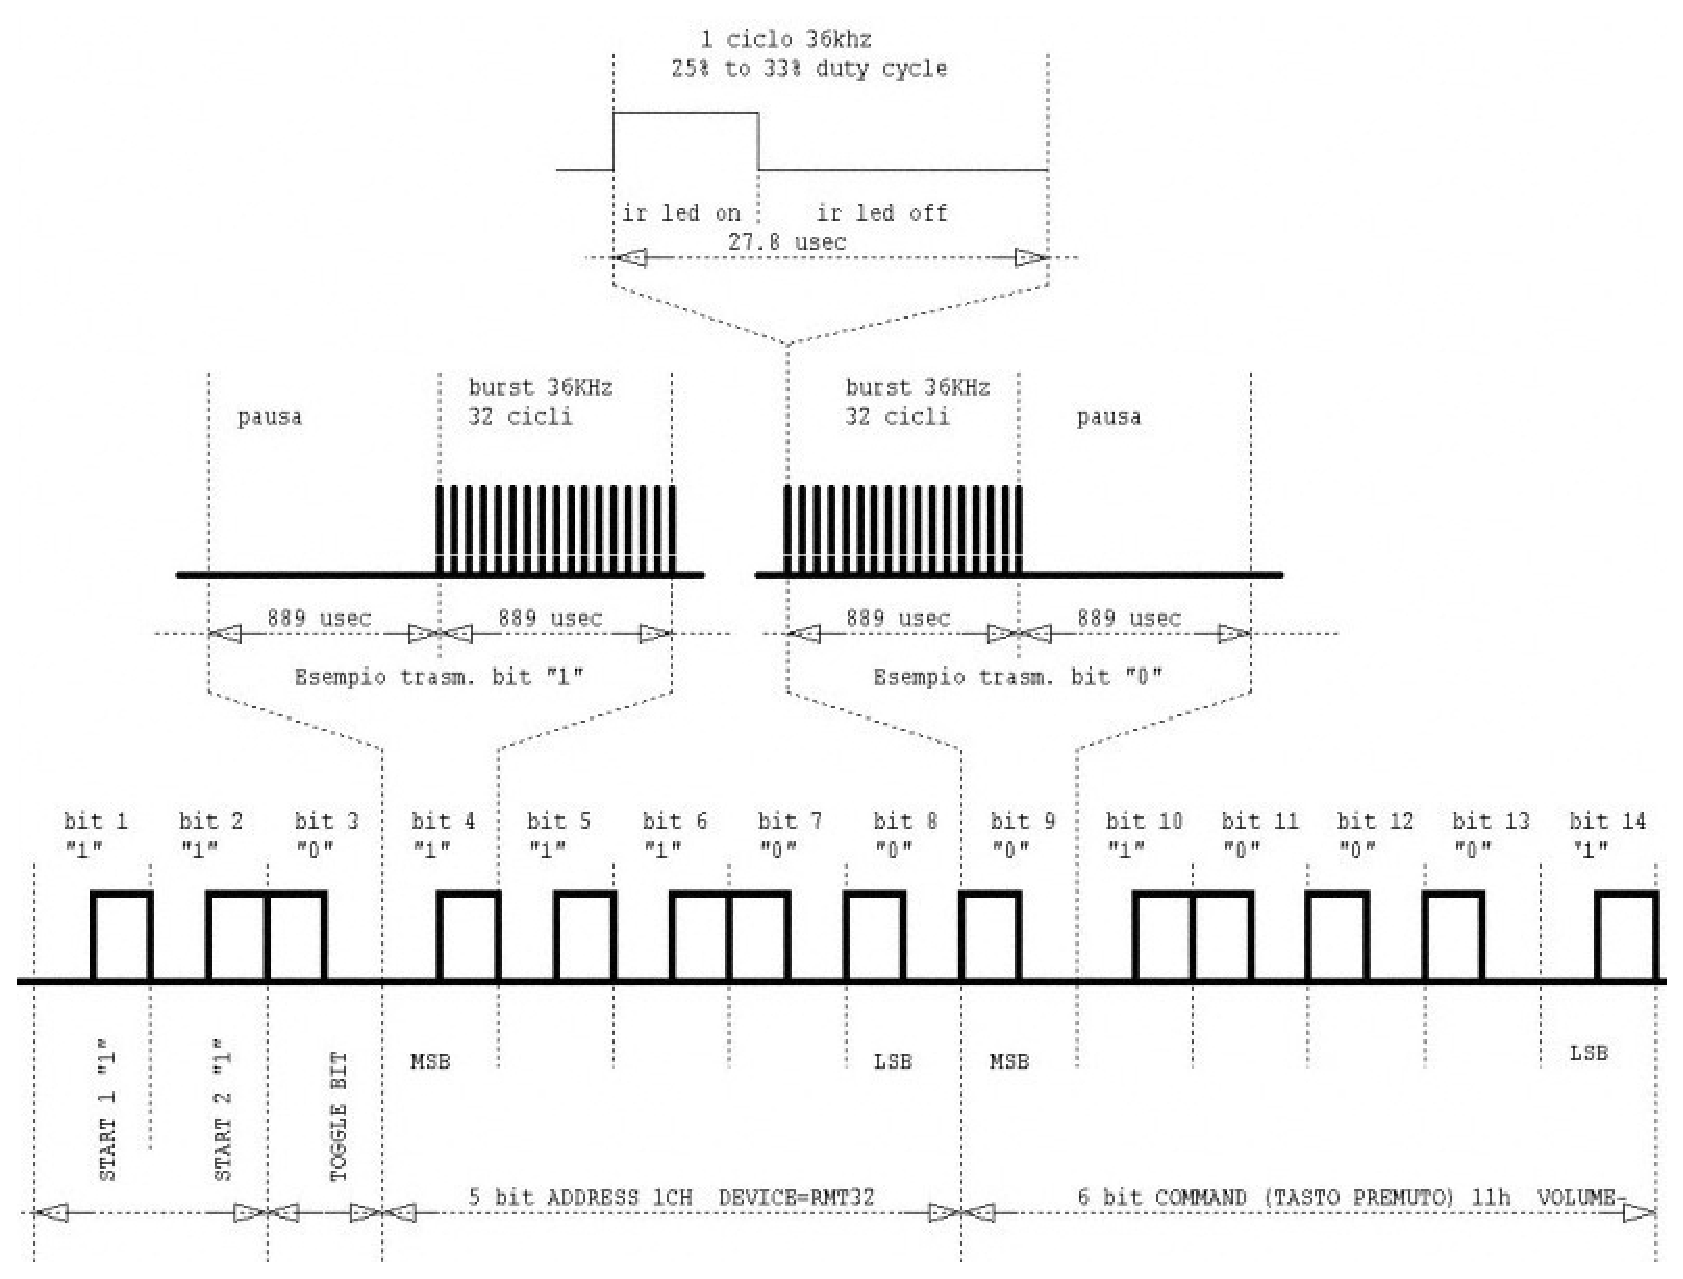
\includegraphics[width=.9\textwidth]{Figures/sch_rc5}
\end{figure}
\end{frame}

\begin{frame}{Protocolo Philips RC-6 (Plot)}
\begin{figure}
	\includegraphics[width=\textwidth]{Figures/cmds}
\end{figure}
\end{frame}

\begin{frame}{Protocolo Samsung}
\begin{figure}
	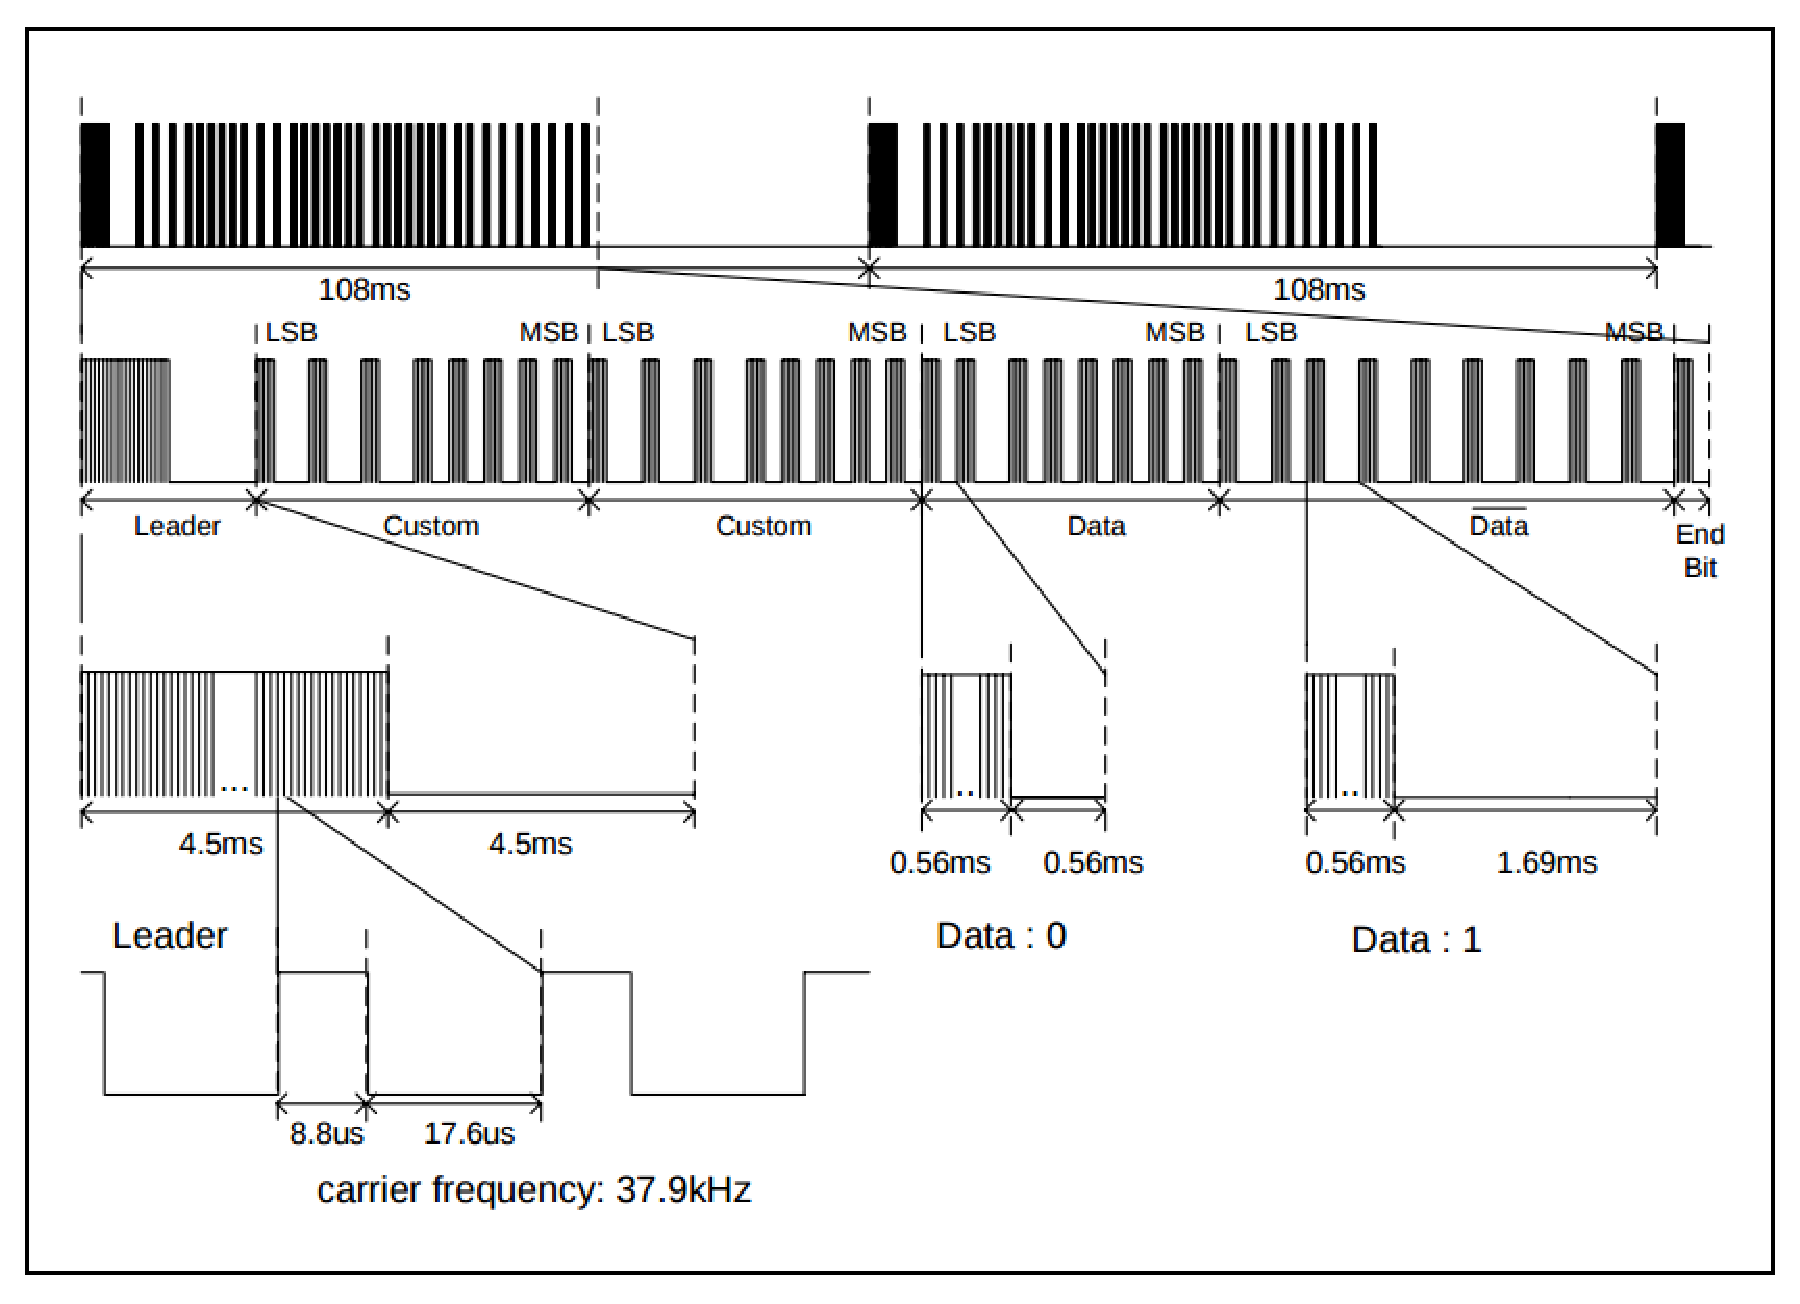
\includegraphics[width=.9\textwidth]{Figures/samsung_protocol}
\end{figure}
\end{frame}

\begin{frame}{Protocolo Samsung (Plot)}
\begin{figure}
	\includegraphics[width=\textwidth]{Figures/cmds_samsung}
\end{figure}
\end{frame}

\section{Work}
\subsection{Work}
\begin{frame}{C�digos, Falhas, Dificuldades...}
\begin{figure}
	
\includegraphics[width=.60\textwidth]{Figures/dificuldades}
\end{figure}
\end{frame}

\begin{frame}{Dificuldades}
\begin{itemize}
	\item Sistema Operacional \smallskip
	\begin{itemize}
		\item �ngstr�m \smallskip
		\item Ubuntu \smallskip
		\item Debian wheezy $\checkmark$ \medskip
	\end{itemize}
	\item Sa�da de �udio\smallskip
	\begin{itemize}
		\item HDMI \smallskip
		\item USB $\checkmark$ \medskip
	\end{itemize}
	\item LibPWM na BeagleBone\smallskip
	\begin{itemize}
		\item DTO: \textit{Device Tree Overlay} \smallskip
		\item Arduino $\checkmark$ \medskip
	\end{itemize}
\end{itemize}
\end{frame}

\begin{frame}{Comunica��o BeagleBone $\rightarrow$ Arduino}
\begin{figure}
	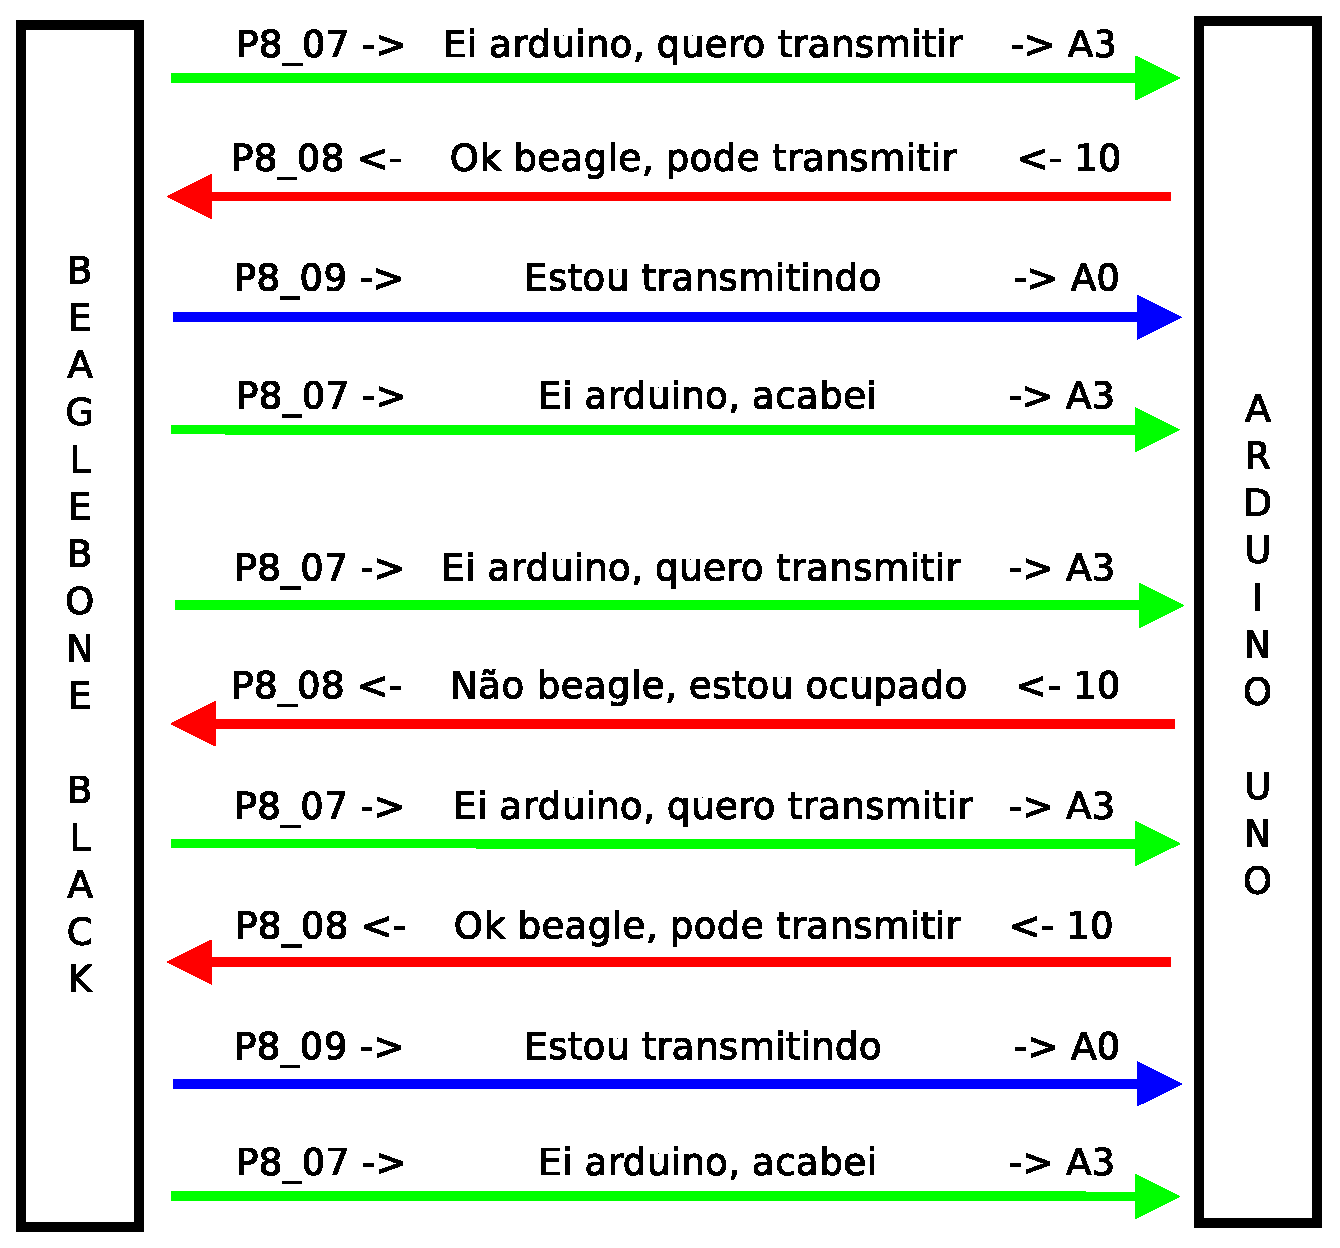
\includegraphics[width=.65\textwidth]{Figures/duplex_tx}
\end{figure}
\end{frame}

\begin{frame}{C�digos}
\begin{itemize}
	\item Protocolo de Comunica��o BBB $\rightarrow$ UNO: \smallskip
	\begin{itemize}
		\item \texttt{DuplexTransmission.ino} \smallskip
		\item \texttt{send2uno.c} \medskip
	\end{itemize}
	\item Banco de Dados (LAMP): \smallskip
	\begin{itemize}
		\item \texttt{db\_phi.c} \smallskip
		\item \texttt{setup\_db.sql} \medskip
	\end{itemize}
\end{itemize}
\end{frame}


\section{Fritzing}
\subsection{Fritzing}
\begin{frame}{Circuito no Fritzing}
\begin{figure}
	\includegraphics[width=.75\textwidth]{Figures/fritzing}
\end{figure}
\end{frame}

%\begin{frame}[fragile]{Comunica��o BeagleBone $\rightarrow$ Arduino}
%\lstinputlisting[language=c,  firstline=36, lastline=65, basicstyle=\tiny\ttfamily]
%{../codes/arduino/DuplexTransmission.ino}
%\end{frame}
%
%\begin{frame}[fragile]{Comunica��o BeagleBone $\rightarrow$ Arduino}
%\lstinputlisting[language=c, firstline=16, lastline=40, basicstyle=\tiny\ttfamily]
%{../codes/bbb/send2uno.c}
%\end{frame}

\section{VLW FLW!}
\begin{frame}{Obrigado!}
\centering
\Huge
Perguntas?
\begin{figure}
	
\includegraphics[width=.30\textwidth]{Figures/question}
\end{figure}
\end{frame}
\end{document}
%%% EOF %%%
